\section{Architecture and Experimental Details}\label{app:architecture}

The causal Grassmann branch uses local past--present pairs, not future-token pairs. A token embedding $h_t\in\mathbb R^d$ is reduced to $z_t=W_{\mathrm{red}}h_t+b_{\mathrm{red}}\in\mathbb R^r$. For $\mathcal D_t=\{\Delta\in\{1,2,4\}:t-\Delta\geq0\}$, the direction is $z_{t-\Delta}\rightarrow z_t$, and the exterior-product coordinates are
\begin{equation}
p_{ij,t}^{(\Delta)}=z_{t,i}z_{t-\Delta,j}-z_{t,j}z_{t-\Delta,i},\quad i<j.
\end{equation}
There are $r(r-1)/2$ coordinates. The subspace background follows basis equivalence on Grassmann manifolds~\citep{edelman1998geometry}. The exterior-product interpretation of Pl\"ucker coordinates is described in the geometric-algebra reference.\footnote{\url{https://cs.uwaterloo.ca/~smann/GA/plucker_coordinates.html}; background only, not evidence about KD.}
Dependent vectors have zero exterior product; normalization remains finite:
\begin{equation}
\widehat p_t^{(\Delta)}=\frac{p_t^{(\Delta)}}{\max(\|p_t^{(\Delta)}\|_2,\epsilon)},\quad\epsilon=10^{-8}.
\end{equation}
Geometric projection precedes the valid-window mean:
\begin{align}
g_t^{(\Delta)}&=W_{\mathrm{plu}}\widehat p_t^{(\Delta)}+b_{\mathrm{plu}},\\
g_t&=\frac{\sum_{\Delta\in\mathcal D_t}g_t^{(\Delta)}}{\max(1,|\mathcal D_t|)}.
\end{align}
An empty window gives zero. Mixing uses a feature-dependent vector gate:
\begin{align}
a_t&=\sigma(W_{\mathrm{gate}}[h_t;g_t]+b_{\mathrm{gate}}),\\
h_t^{\mathrm{mix}}&=a_t\odot h_t+(1-a_t)\odot g_t.
\end{align}
LayerNorm, dropout, and residual feed-forward processing surround this core. The LM head produces G logits independently of the Transformer logits; scalar $\alpha$ applies only at late fusion (Equation~\ref{eq:teacher-fusion}). Figure~\ref{fig:teacher_architecture} is generic and does not fix $\alpha=0.5$.

The compact primary student uses six layers, width 224, eight Transformer heads, reduced width 56, dropout 0.1, and final-block fusion. It has 31,434,257 parameters. The local GPT-2 tokenizer has vocabulary size 50,257 without added special tokens. Teacher dimensions and states follow their source configurations, not the student dimensions. The architecture is an existing test bed, not a geometry-specific method contribution.

\begin{figure*}[!t]
\centering
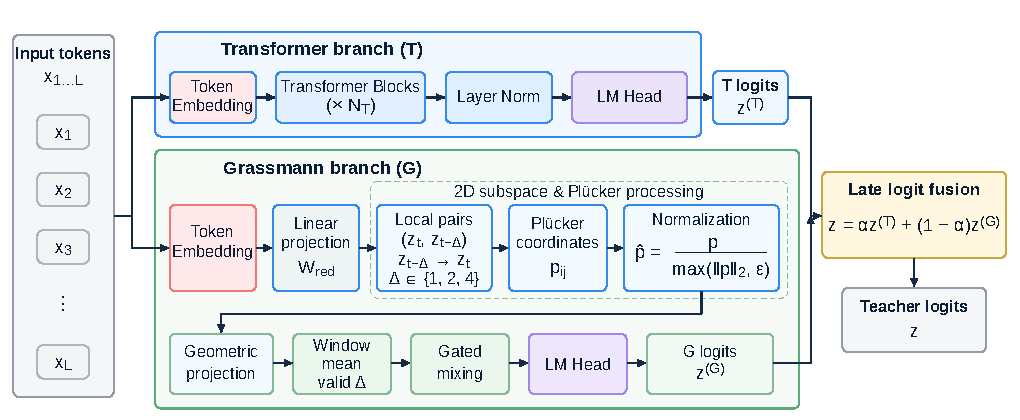
\includegraphics[width=\textwidth]{figures/figA1_teacher_architecture.pdf}
\caption{Generic heterogeneous teacher. The Grassmann path uses causal local pairs, normalized Pl\"ucker coordinates, geometric projection, valid-window averaging, gated mixing, and an LM head. Late fusion acts on logits with free $\alpha$. The architecture does not establish geometric KD superiority.}
\label{fig:teacher_architecture}
\end{figure*}
